% >8-----------------------------ESTRUTURAS DE DADOS EM LUA------------------------------8<
\section{Tabelas Hash}
\begin{frame}
  \frametitle{Tabelas Hash em Lua}
  \begin{center}
    \textit{Tables are the main (in fact, the only) data structuring \\
              mechanism in Lua, and a powerful one. We use tables to \\
              represent [...] data structures in a simple, uniform, \\
              and efficient way.}\\
        --- Roberto Ierusalimschy.
    \end{center}
\end{frame}

\begin{frame}
  \frametitle{Tabelas Hash em Lua}
  \begin{figure}
    \centering
    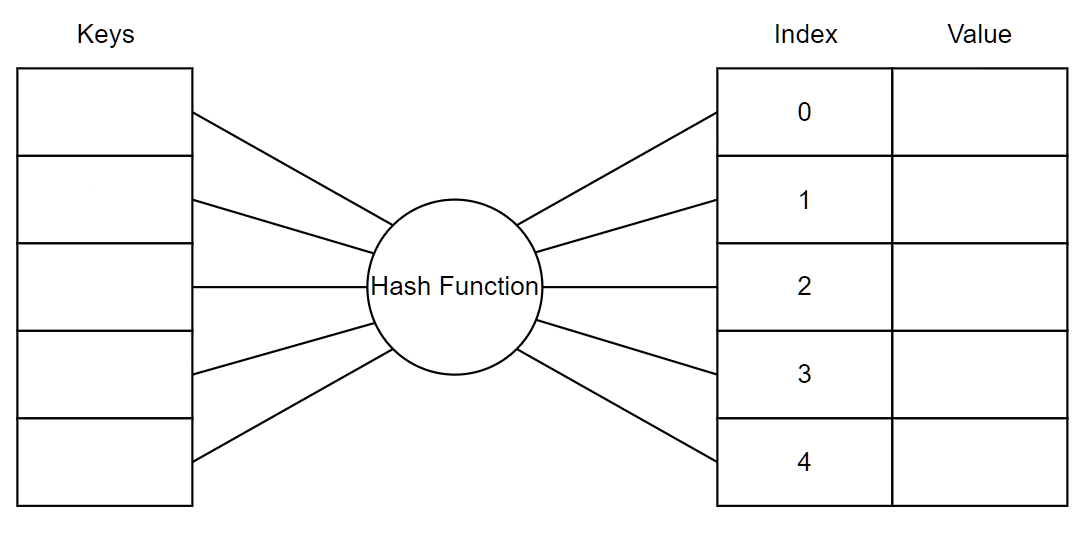
\includegraphics[width=0.8\linewidth]{hash-1.png}
  \end{figure}
\end{frame}


\begin{frame}[fragile]
  \frametitle{Estruturas de Dados a partir de tabelas hash}

  \begin{code}
local array = {}  -- create the "array"

for i = 1, 1000 do
  array[i] = 0
end
  \end{code}
\end{frame}

\begin{frame}[fragile]
  \frametitle{Estruturas de Dados a partir de tabelas hash}
  \begin{code}
local matrix = {} -- create the "matrix"

for i = 1, N do
  local row = {}  -- create a new "row"
  matrix[i] = row
end
  \end{code}
\end{frame}

\begin{frame}[fragile]
  \frametitle{Estruturas de Dados a partir de tabelas hash}
  \begin{code}
list = nil -- create the "list"

list = {value = v, next = list} -- create a new "list"
  \end{code}
% local l = list
% while l do -- traverse the list
%   visit l.value
%   l = l.next
% end
\end{frame}

% >8-----------------------------ESTRUTURAS DE DADOS EM LUA------------------------------8<